\section{ARMA process}

We can define a process that combines elements from both the AutoRegressive and Moving Average processes as follows:
\[y(t)=a_1y(t-1)+a_2y(t-2)+\cdots+a_m y(t-m)+c_0e(t)+c_1e(t-1)+\cdots+c_n e(t-n) \]
Here, $e(t)\sim WN(0,\lambda^2)$.

This process comprises two components: one being the AR($m$) process and the other being the MA($n$) process. 
It is denoted as an ARMA($m,n$) process.
Since it combines elements from two distinct processes, we can make the following observations:
\begin{itemize}
    \item The MA($n$) process is equivalent to an ARMA($0,n$) process.
    \item The AR($m$) process is equivalent to an ARMA($m,0$) process. 
\end{itemize}
\begin{figure}[H]
    \centering
    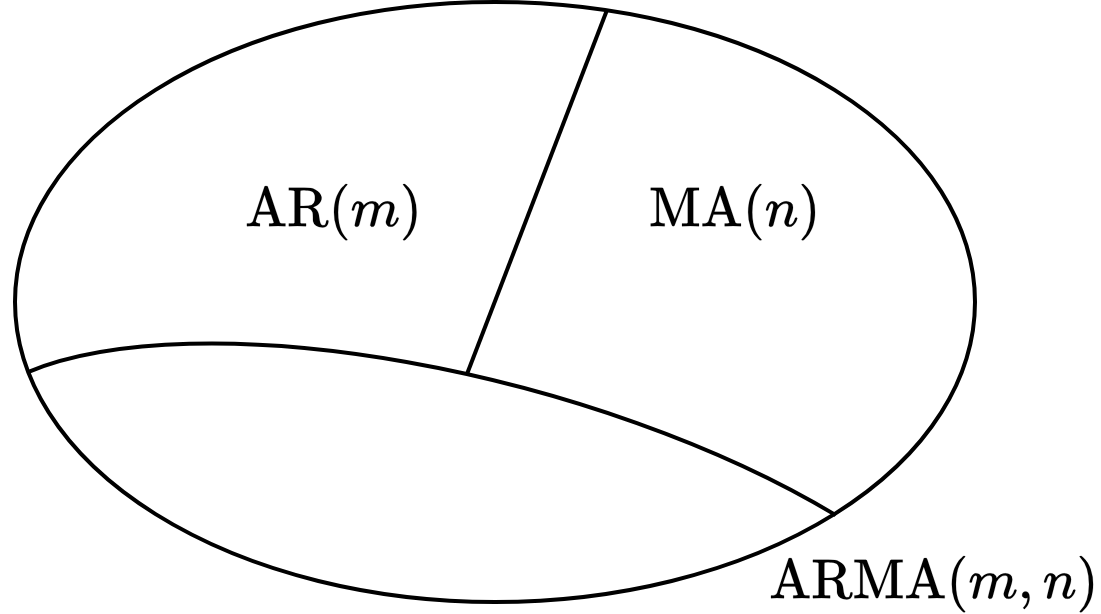
\includegraphics[width=0.45\linewidth]{images/set.png}
    \caption{Inclusion of ARMA processes}
\end{figure}

\subsection{Operatorial representation}
Given an ARMA($m,n$) process defined as:
\[y(t)=a_1y(t-1)+a_2y(t-2)+\cdots+a_m y(t-m)+c_0e(t)+c_1e(t-1)+\cdots+c_n e(t-n)\]
Here, $e(t)\sim WN(0,\lambda^2)$.

We can rewrite it using operatorial representation as:
\[y(t)=a_1z^{-1}y(t)+a_2z^{-2}y(t)+\cdots+a_m z^{-m}y(t)+c_0e(t)+c_1z^{-1}e(t)+\cdots+c_n z^{-n}e(t)\]
Rearranging terms, we get:
\[\left(1- a_1z^{-1}-a_2z^{-2}-\cdots-a_m z^{-m}\right)y(t)=\left(c_0+c_1z^{-1}+\cdots+c_n z^{-n}\right)e(t)\]
Finally, we can express $y(t)$ in terms of $e(t)$ using the transfer function notation:
\[y(t)=\dfrac{c_0+c_1z^{-1}+\cdots+c_n z^{-n}}{1- a_1z^{-1}-a_2z^{-2}-\cdots-a_m z^{-m}}e(t)=\dfrac{C(z)}{A(z)}e(t)\]
Here, $C(z)$ and $A(z)$ are polynomials representing the coefficients of the Moving Average and AR parts, respectively. 
This ratio, denoted as $W(z)$, is a discrete-time transfer function. 
This operator acts as a digital filter, transforming the input noise sequence $e(t)$ into the output sequence $y(t)$.

\subsection{Mean value}
Given an ARMA($m,n$) model defined as:
\[y(t)=a_1y(t-1)+a_2y(t-2)+\cdots+a_m y(t-m)+c_0e(t)+c_1e(t-1)+\cdots+c_n e(t-n)\]
where $e(t)\sim WN(0,\lambda^2)$, we can compute its mean as follows:
\begin{align*}
    \mathbb{E}\left[y(t)\right] &= \mathbb{E}\left[a_1y(t-1)+\cdots+a_m y(t-m)+c_0e(t)+\cdots+c_n e(t-n)\right] \\
                                &= a_1\mathbb{E}\left[y(t-1)\right]+\cdots+a_m\mathbb{E}\left[y(t-m)\right] +c_0\underbrace{\mathbb{E}\left[e(t)\right]}_0 +\cdots+c_n\underbrace{\mathbb{E}\left[e(t-n)\right]}_0
\end{align*}
Under the assumption that $a_1,a_2,\dots,a_m$ are chosen such that $y(t)$ constitutes a stationary stochastic process, thus exhibiting a constant mean value, we can simplify the above to:
\[m_y=a_1m_y+a_2m_y+\cdots+a_m m_y \rightarrow m_y=0\]

\subsection{Covariance function}
Given an ARMA($m,n$) model defined as:
\[y(t)=a_1y(t-1)+a_2y(t-2)+\cdots+a_m y(t-m)+c_0e(t)+c_1e(t-1)+\cdots+c_n e(t-n)\]
where $e(t)\sim WN(0,\lambda^2)$, we aim to compute the covariance function at $\tau=0$, considering $m_y=0$:
\begin{align*}
    \gamma_y(0) &=\mathbb{E}\left[ \left(y(t)-m_y\right)\left(y(t)-m_y\right) \right] \\
                &=\mathbb{E}\left[ {\left(y(t)\right)}^2 \right] \\
                &=\mathbb{E}\left[ {\left(a_1y(t-1)+\cdots+a_m y(t-m)+c_0e(t)+\cdots+c_n e(t-n)\right)}^2 \right] \\      
                &=a_1^2\underbrace{\mathbb{E}\left[ {y(t-1)}^2 \right]}_{\gamma_y(0)} +\cdots+c_0^2\underbrace{\mathbb{E}\left[ {e(t)}^2 \right]}_{\lambda^2} +\cdots+c_n^2 \underbrace{\mathbb{E}\left[ {e(t-n)}^2 \right]}_{\lambda^2}  +\\
                &+ 2a_1a_2\underbrace{\mathbb{E}\left[ y(t-1)y(t-2) \right]}_{\gamma_y(1)}  + \cdots + 2a_1c_0\underbrace{\mathbb{E}\left[ y(t-1)e(t) \right]}_{0 \text{ if the times are different}}  + \cdots + 2c_0c_1\underbrace{\mathbb{E}\left[ e(t)e(t-1) \right]}_0  \\   
                &=a_1^2\gamma_y(0) +\cdots+c_0^2\lambda^2 +\cdots+c_n^2 \lambda^2  + 2a_1a_2\gamma_y(1)  + \cdots + 2a_1c_1\mathbb{E}\left[ y(t-1)e(t-1) \right]+\dots    
\end{align*}
We require $\gamma_y(1),\gamma_y(2),\dots,\gamma_y(n)$ to compute $\gamma_y(0)$.

To compute the covariance function at $\tau=1$, considering $m_y=0$, we have:
\begin{align*}
    \gamma_y(1) &=\mathbb{E}\left[ \left(y(t)-m_y\right)\left(y(t-1)-m_y\right) \right] \\
                &=\mathbb{E}\left[ \left(a_1y(t-1)+\cdots+a_m y(t-m)+c_0e(t)+\cdots+c_n e(t-n)\right)y(t-1) \right] \\
                &=a_1\mathbb{E}\left[{y(t-1)}^2\right]+\cdots+c_0\mathbb{E}\left[e(t)y(t-1)\right]+\dots \\
                &=a_1\gamma_y(0)+\cdots+c_0\mathbb{E}\left[e(t)y(t-1)\right]+\dots
\end{align*}
Proceeding with increasing values of $\tau$, we obtain a set of $m$ recursive equations known as Yule-Walker equations for an ARMA($m,n$) process:
\[\begin{cases}
    \gamma_y(0)=a_1^2\gamma_y(0) +a_2^2\gamma_y(0) +2a_1a_2\gamma_y(1) +\dots \\
    \gamma_y(1)=a_1\gamma_y(0) +c_0\mathbb{E}\left[e(t)y(t-1)\right] +\dots \\
    \vdots \\
    \gamma_y(m-1)=a_1\gamma_y(m-2)+\dots
\end{cases}\]
At the end we get a set of $m$ recursive equations called Yule-Walker equations for an ARMA($m,n$) process.
These equations require all covariances $\gamma_y(0),\gamma_y(1),\dots,\gamma_y(m-1)$ to compute $\gamma_y(m)$.